\documentclass{article}
\usepackage[margin=1in]{geometry}
\usepackage{amsmath,amsfonts,amssymb}
\usepackage{listings}
\usepackage{color}
\usepackage{graphicx}
\usepackage{subfig}
\usepackage{blkarray}
\usepackage{multirow}
\usepackage{float}
\usepackage{caption}
\usepackage{subcaption}
\begin{document}
\begin{titlepage}
	\setlength{\parindent}{0pt}
	\large

\vspace*{-2cm}

\definecolor{dkgreen}{rgb}{0,0.6,0}
\definecolor{gray}{rgb}{0.5,0.5,0.5}
\definecolor{mauve}{rgb}{0.58,0,0.82}

\lstset{frame=tb,
  language=Python,
  aboveskip=3mm,
  belowskip=3mm,
  showstringspaces=false,
  columns=flexible,
  basicstyle={\small\ttfamily},
  numbers=none,
  numberstyle=\tiny\color{gray},
  keywordstyle=\color{blue},
  commentstyle=\color{dkgreen},
  stringstyle=\color{mauve},
  breaklines=true,
  breakatwhitespace=true,
  tabsize=3
}

University of Waterloo \par
CS 480 \par
\vspace{0.05cm}
r2knowle: 2023-11-13
\vspace{0.2cm}

{\huge Exercise \# 2 \par}
\hrule

\vspace{0.5cm}
\textbf{Q2b)} Below are the 4 graphs each documenting an aspect of the training and testing process for our VG11 net implimention:

\begin{tabular}{ll}

 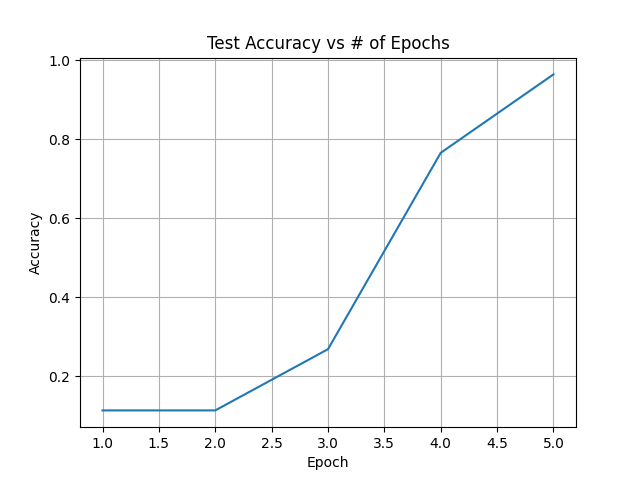
\includegraphics[width=.5\linewidth]{testA.png} &  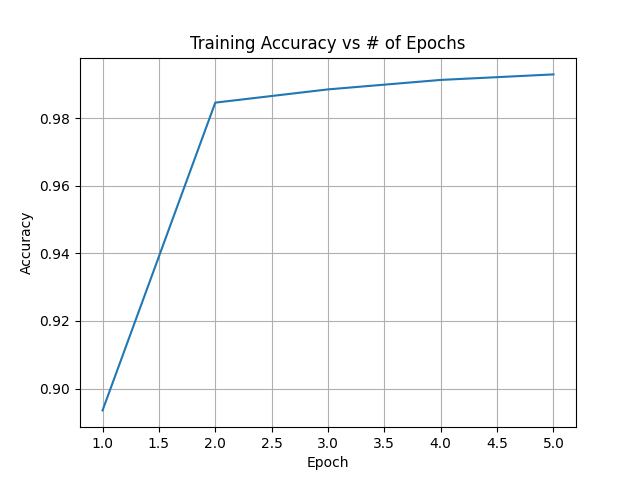
\includegraphics[width=.5\linewidth]{trainA.png}\\
 \hfil (i) Test accuracy vs the number of epochs \hfil & \hfil (ii) Training accuracy vs the number of epochs \hfil \\
 
  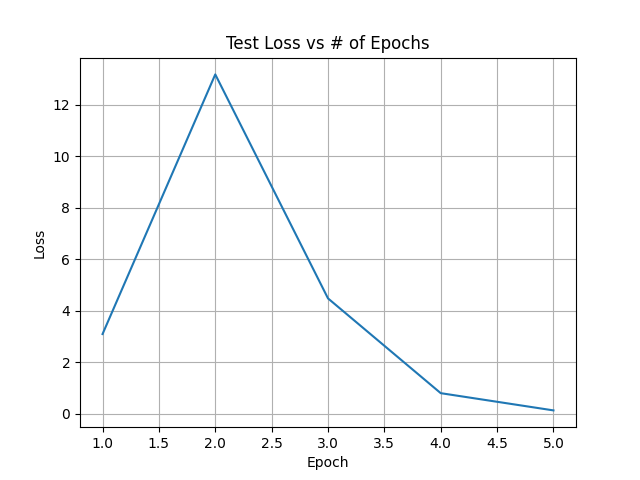
\includegraphics[width=.5\linewidth]{testL.png} &  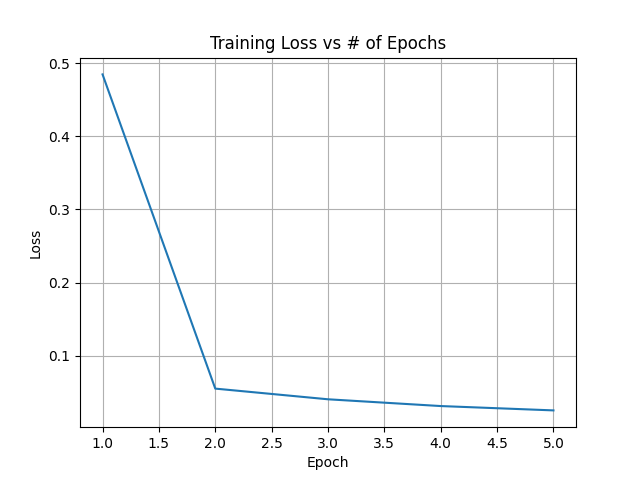
\includegraphics[width=.5\linewidth]{trainL.png}\\
 \hfil (i) Test loss vs the number of epochs \hfil & \hfil (ii) Training loss vs the number of epochs \hfil 
 
\end{tabular}
\newpage
\textbf{Q2ci)} Below we can see the testing accuracy across each flip:
\begin{center} 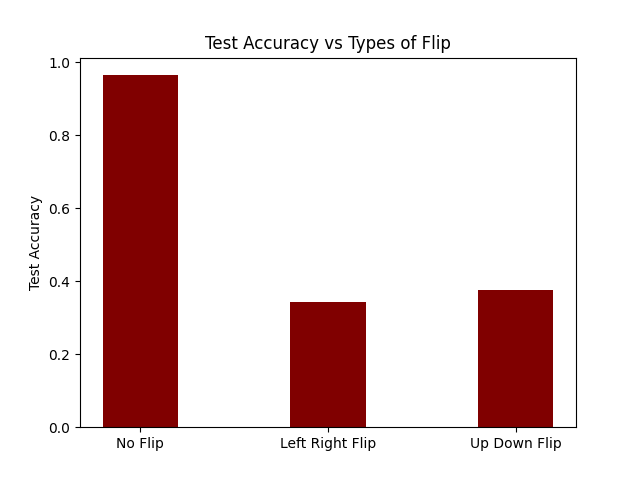
\includegraphics[width=0.7\linewidth]{flip.png} 
\end{center}
We can see that the updown flip has a higher testing accuracy then the left-right flip, this can be due to the fact that some digits remain more unchanged (like 3) from an updown flip then a right left flip. \textbf{Explict values are provided on the next page. } \\\\
\textbf{Q2cii)} Below we can see the testing accuracy across each flip:
\begin{center} 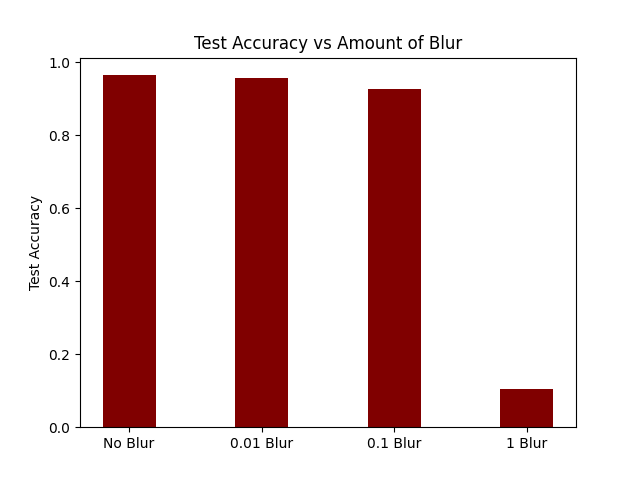
\includegraphics[width=0.7\linewidth]{blur.png} 
\end{center}
As the amount of blur increases, we can see that testing accuracy decreases. \textbf{Explict values are provided on the next page. }
\newpage
\textbf{Q2d)} By applying the both times of flips, and 0.01 and 0.1 blurring to our original dataset we can retrain for 5 epochs. After which we get the following graphs.\\
\begin{tabular}{ll}

 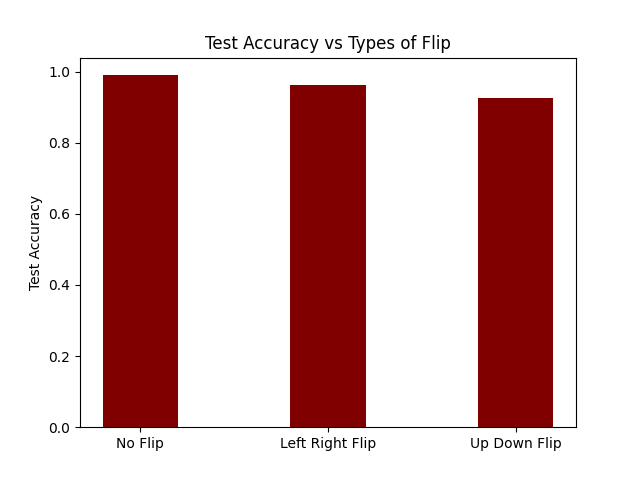
\includegraphics[width=.5\linewidth]{flip2.png} &  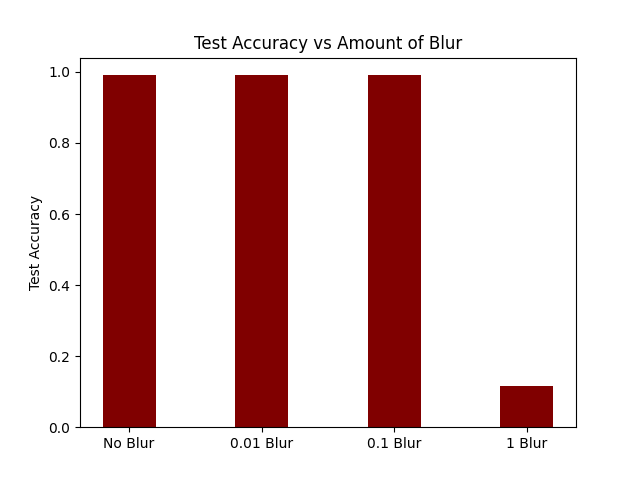
\includegraphics[width=.5\linewidth]{blur2.png}\\
 \hfil (i) Test accuracy vs flips \hfil & \hfil (ii) Training accuracy vs blur \hfil \\\\
 
\end{tabular}
We get the following updated test accuracies:
\begin{enumerate}
  \item No Flip / No Blur: 0.9899
  \item Left Right Flip: 0.9635
  \item Up Down Flip: 0.9255
  \item 0.01 Blur: 0.9905
  \item 0.1 Blur: 0.9907
  \item 1 Blur: 0.1159
\end{enumerate}
This is comparison to before we did the retraining where we had the following test accuracies:
\begin{enumerate}
  \item No Flip / No Blur: 0.9784
  \item Left Right Flip: 0.3481
  \item Up Down Flip: 0.3755
  \item 0.01 Blur: 0.9705
  \item 0.1 Blur: 0.9503
  \item 1 Blur: 0.1139
\end{enumerate}
\newpage
Below is the code used for this question:
\begin{lstlisting}
import tensorflow as tf
import numpy as np
import matplotlib.pyplot as plt
import pandas as pd

from tensorflow.keras import layers, models


# ==================== Import MNIST dataset and Normalize ====================

def normalize_img(image):
    scaled_image = image / 255.  # Scale the image to 0-1

    # Add the top padding to the image
    top = np.zeros((2, 28))
    bottom = top
    image32By28 = np.concatenate([top, scaled_image, bottom], 0)

    left = np.zeros((32, 2))
    right = left
    finalImage = np.concatenate([left, image32By28, right], 1)

    return finalImage  # Return image with label


(x_train, y_train), (x_test, y_test) = tf.keras.datasets.mnist.load_data()


updated_train = []
updated_test = []

for i in range(0, len(x_train)):
    updated_train.append(normalize_img(x_train[i]))

for i in range(0, len(x_test)):
    updated_test.append(normalize_img(x_test[i]))


leftRight = []
upDown = []
for i in range(0, len(updated_train)):          # Generate Left Right Flip
    leftRight.append(np.fliplr(updated_train[i]))

for i in range(0, len(updated_train)):          # Generate Up Down Flip
    upDown.append(np.flipud(updated_train[i]))

var1 = []
var2 = []

for i in range(0, len(updated_train)):           # Generate 0.01 Blur
    newDataPoint = []
    for row in updated_train[i]:
        newRow = []
        for element in row:
            element += np.random.normal(0,0.01)
            newRow.append(element)
        newDataPoint.append(newRow)
    var1.append(newDataPoint)

for i in range(0, len(updated_train)):           # Generate 0.1 Blur
    newDataPoint = []
    for row in updated_train[i]:
        newRow = []
        for element in row:
            element += np.random.normal(0,0.1)
            newRow.append(element)
        newDataPoint.append(newRow)
    var2.append(newDataPoint)

var1 = np.array(var1)
var2 = np.array(var2)
leftRight = np.array(leftRight)
upDown = np.array(upDown)

updated_train = np.array(updated_train)
updated_test = np.array(updated_test)

# Combine all of them datasets
updated_train = np.concatenate((updated_train, leftRight, upDown, var1, var2), axis=0)
y_train = np.concatenate((y_train, y_train, y_train, y_train, y_train), axis=0)

# ==================== Model Definition ====================

model = models.Sequential()

model.add(
    layers.Conv2D(filters=64, kernel_size=3, strides=1, padding="same", activation='relu', input_shape=(32, 32, 1)))
model.add(layers.BatchNormalization())
model.add(layers.MaxPooling2D(pool_size=(2, 2), padding="same"))

model.add(layers.Conv2D(filters=128, kernel_size=3, strides=1, padding="same", activation='relu'))
model.add(layers.BatchNormalization())
model.add(layers.MaxPooling2D(pool_size=(2, 2), padding="same"))

model.add(layers.Conv2D(filters=256, kernel_size=3, strides=1, padding="same", activation='relu'))
model.add(layers.BatchNormalization())

model.add(layers.Conv2D(filters=256, kernel_size=3, strides=1, padding="same", activation='relu'))
model.add(layers.BatchNormalization())
model.add(layers.MaxPooling2D(pool_size=(2, 2), padding="same"))

model.add(layers.Conv2D(filters=512, kernel_size=3, strides=1, padding="same", activation='relu'))
model.add(layers.BatchNormalization())

model.add(layers.Conv2D(filters=512, kernel_size=3, strides=1, padding="same", activation='relu'))
model.add(layers.BatchNormalization())
model.add(layers.MaxPooling2D(pool_size=(2, 2), padding="same"))

model.add(layers.Conv2D(filters=512, kernel_size=3, strides=1, padding="same", activation='relu'))
model.add(layers.BatchNormalization())

model.add(layers.Conv2D(filters=512, kernel_size=3, strides=1, padding="same", activation='relu'))
model.add(layers.BatchNormalization())
model.add(layers.MaxPooling2D(pool_size=(2, 2), padding="same"))
model.add(layers.Flatten())

model.add(layers.Dense(4096, activation='relu'))
model.add(layers.Dropout(.5))

model.add(layers.Dense(4096, activation='relu'))
model.add(layers.Dropout(.5))

model.add(layers.Dense(10))

# ==================== Training and Testing ====================

model.compile(
    optimizer=tf.keras.optimizers.Adam(),
    loss=tf.keras.losses.SparseCategoricalCrossentropy(from_logits=True),
    metrics=[tf.keras.metrics.SparseCategoricalAccuracy()],
)
trainingAccuracy = []
trainingLoss = []

testAccuracy = []
testLoss = []

for i in range(0, 5):
    history = model.fit(updated_train, y_train, epochs=1, batch_size=512)

    trainingAccuracy.append(history.history["sparse_categorical_accuracy"][0])
    trainingLoss.append(history.history["loss"][0])

    test_loss, test_acc = model.evaluate(updated_test, y_test, verbose=1)

    testAccuracy.append(test_acc)
    testLoss.append(test_loss)
    model.save('q3TrainedExtra'+str(i)+'.keras')

# ==================== Graphing ====================
x = []
for i in range(0, len(testAccuracy)):
    x.append(i+1)

plt.plot(x, trainingAccuracy)
plt.title('Training Accuracy vs # of Epochs')
plt.ylabel('Accuracy')
plt.xlabel('Epoch')
plt.grid()
plt.show()

plt.plot(x, trainingLoss)
plt.title('Training Loss vs # of Epochs')
plt.ylabel('Loss')
plt.xlabel('Epoch')
plt.grid()
plt.show()

plt.plot(x, testAccuracy)
plt.title('Test Accuracy vs # of Epochs')
plt.ylabel('Accuracy')
plt.xlabel('Epoch')
plt.grid()
plt.show()

plt.plot(x, testLoss)
plt.title('Test Loss vs # of Epochs')
plt.ylabel('Loss')
plt.xlabel('Epoch')
plt.grid()
plt.show()

trainedModel = tf.keras.models.load_model('q3TrainedExtra4.keras')

_, test_acc = trainedModel.evaluate(updated_test, y_test, verbose=1)

leftRight = []
upDown = []
for i in range(0, len(updated_test)):
    leftRight.append(np.fliplr(updated_test[i]))

for i in range(0, len(updated_test)):
    upDown.append(np.flipud(updated_test[i]))

leftRight = np.array(leftRight)
upDown = np.array(upDown)

_, test_acc_lr = trainedModel.evaluate(leftRight, y_test, verbose=1)
_, test_acc_ud = trainedModel.evaluate(upDown, y_test, verbose=1)

print(test_acc)
print(test_acc_lr)
print(test_acc_ud)

plt.bar(["No Flip", "Left Right Flip", "Up Down Flip"], [test_acc, test_acc_lr, test_acc_ud], color ='maroon',
        width = 0.4)
plt.ylabel("Test Accuracy")
plt.title("Test Accuracy vs Types of Flip")
plt.show()

var1 = []
var2 = []
var3 = []

for i in range(0, len(updated_test)):
    newDataPoint = []
    for row in updated_test[i]:
        newRow = []
        for element in row:
            element += np.random.normal(0,0.01)
            newRow.append(element)
        newDataPoint.append(newRow)
    var1.append(newDataPoint)

for i in range(0, len(updated_test)):
    newDataPoint = []
    for row in updated_test[i]:
        newRow = []
        for element in row:
            element += np.random.normal(0,0.1)
            newRow.append(element)
        newDataPoint.append(newRow)
    var2.append(newDataPoint)

for i in range(0, len(updated_test)):
    newDataPoint = []
    for row in updated_test[i]:
        newRow = []
        for element in row:
            element += np.random.normal(0,1)
            newRow.append(element)
        newDataPoint.append(newRow)
    var3.append(newDataPoint)

var1 = np.array(var1)
var2 = np.array(var2)
var3 = np.array(var3)

_, test_acc_var1 = trainedModel.evaluate(var1, y_test, verbose=1)
_, test_acc_var2 = trainedModel.evaluate(var2, y_test, verbose=1)
_, test_acc_var3 = trainedModel.evaluate(var3, y_test, verbose=1)

plt.bar(["No Blur", "0.01 Blur", "0.1 Blur", "1 Blur"], [test_acc, test_acc_var1, test_acc_var2, test_acc_var3], color ='maroon',
        width = 0.4)
plt.ylabel("Test Accuracy")
plt.title("Test Accuracy vs Amount of Blur")
plt.show()
print(test_acc_var1)
\end{lstlisting}
\end{titlepage}
\end{document}